\section{Introduction}
\label{sec:soa_intro}

% no habría que definir de nuevo y de manera formal ubicomp o vale con la intro?
Due to the heterogeneity of technologies present in \ac{ubicomp} environments, % computing platforms, protocols, etc.
our solution should carefully consider the \emph{interoperability}.
The IEEE defines interoperability as \emph{the ability of two or more systems or components to exchange information and to use the information that has been exchanged}.
The definition clearly distinguishes between two requirements: % o goals o incremental requirements
(1) to exchange information (i.e. \emph{integration}); and
(2) to use that information. % to understand others data (i.e. \emph{interoperation}).


% Buscar una referencia mejor: http://en.wikipedia.org/wiki/Interoperability
For the lower-levels of the exchange, we opt for interoperability \emph{ab-initio} relying in standard and widely accepted communication protocols. % e.g. HTTP
For a higher-level (i.e. application layer), Section~\ref{} categorizes integration approaches and describes the ones explored in this dissertation.

% Sintáctica vs semántica
Regarding the second goal, 
Section~\ref{} stresses the need of the \acl{sw} for these environments.

% interoperability. The ability of two or more systems or components to exchange information and to use the information that has been exchanged

% Poner primero el ejemplo motivacional
% \subsection{A closer look to application-level Interoperability}
\label{sec:closer}

% TODO mejor que listar "lo que un developer" debería hacer, listarlo mejor como requisitos para que 2 aplicaciones YA existentes puedan usar datos las una de la otra.
A developer using \ac{ts} could try to reuse the data from another \emph{application A}.
% Let us imagine an \emph{application A} where some devices (masters) write tasks of the same type in a space.
% For the same application, some other devices (workers) take each tuple representing the task, perform the task, and write the result in the same space.
% Providing that a new \emph{application B} needs the same type of task to be done, a clever can try to reuse the work done by the workers.
%To take advantage of these workers already implemented and deployed, he needs to:
To do that he should:
\begin{itemize}
 \item Use the same space.% as the \emph{application A}.
 \item Read the results by using a proper template.
	Therefore, he needs to know the format of the tuples written by \emph{application A}.
 \item Write the information in the same format, if he wants to enable two-way interoperability
      (i.e. allow \emph{application A} consume the new application's data).
      % For that, he should be able to figure out the kind of tuple a worker consumes.

\end{itemize}

While the first step may be trivial, the second and third steps require the developer to carefully study the \emph{application A}.
%Specifically, he needs to know the number and the type of fields of the tuples which represent a task and a result.
Since this process is inherently manual, it is a stumbling block to achieve application-level interoperability.

\medskip

Similarly, for each application willing to reuse other application's service in \ac{wot}, a developer should know:
\begin{itemize}
 \item The URL.
 \item The media-types it returns or it accepts as input.
 \item For an specific media-type, the syntax of the result provided by the service or the data provided to the service. % e.g. URL
\end{itemize}

% On the other hand, most of the solutions in the \ac{wot} use common web media formats such as HyperText Markup Language (HTML) or JavaScript Object Notation (JSON). % link
% HTML is oriented for humans while JSON is a machine processable format.
% Imagine a developer wants to regulate the brightness of a room by using some existing and already deployed \acs{wot}-enabled devices.
% A device provides temperature through a REST \emph{service A} and other device has a REST \emph{service B} to switch on or switch off the lights.
% Then, the developer will need to know:
% \begin{itemize}
%  \item The URL of the service A which provides the temperature.
%  \item The URL of the service B which controls the lights of the room.
%  \item The media-types that the service A returns.
%  \item The media-types that the service B accepts.
%  \item Once he has chosen a media-type, the syntax of the result provided by the service A.
%  \item Once he has chosen a media-type, the syntax of the piece of data the service B is able to interpret.
% \end{itemize}

The first step requires the developer to browse and identify the key services.
This identification needs of a human interpretation unless the services provide some semantics in their description. % RESTdesc
The remaining steps require the developer to study each service to create and send or receive and interpret each piece of data.

Furthermore, the different services will be hardly exchangeable.
Let us imagine that there is an hypothetical temperature regulation application which uses the data acquired from a temperature sensor.
This sensor provides the data in a RESTful manner.
Now, let us imagine that somebody replaces the sensor with a new one used in a third application.
Let us assume that the service which will now return the temperature uses the same URL and returns the same media-type as the previous one.
Even in that case, if the second device provides the temperature using a different syntax, the application will not work anymore.

\medskip

% TODO poner ejemplo de interoperabilidad para enganchar con lo de arriba? ponerlo directamente arriba?

% no me acaba de convencer este parrafo introductorio
In conclusion, the systems analyzed in the previous section use information not meaningful for other applications or domains.
One solution to that problem is to use specialized systems which convert and reinterpret the data from one domain to the other.
Other one is to promote the use of standardized models to express the data.
In the next section we will analyze how the \acl{sw} tackles these problems. % <- no vale mucho

% SECCIÓN: CÓMO MOLA Y FUNCIONA NUESTRA IMPLEMENTACIÓN, QUE ES EL FOCO DEL PAPER
% 
% TODO: Poner que a pesar de que el ejemplo descrito no es real ha sido for the sake of clarity, pero 
% que el sistema ha sido utilizado en supermercados y hospitales reales como está descrito en [1] noticia en castellano [2] paper nuestro hablando de ello en otra confe pasada
% 
\section{Case study}

Otsopack has been used in real scenarios both in a supermarket and in a hospital with more complex applications within
the ACROSS project\footnote{\url{http://www.acrosspse.com/across/servlet/Noticias?id=33}\linebreak
\url{http://www.acrosspse.com/across/servlet/Noticias?id=35}}. For the sake of brevity and clarity, two simple and not
implemented applications have been designed for this contribution. The aim of them is to show how the middleware
solution can be used to achieve interoperability. In order to prove the feasibility of the implementation in limited
devices, times measured in real sensors are used.

For the case study, we will model two different applications: \textit{otsoSecurity} and \textit{otsoHomeAutomation},
which have not been implemented.

\subsection{Security}

A security company can develop an application which monitors different parameters such as the temperature, the humidity
or the $CO_2$ concentration with different sensors deployed over an industrial facility. Whenever any of this measures
go
beyond a determined threshold, the company needs to take the proper action. To answer to the potential risks the
application
creates tasks with different priorities: when a unimportant parameter is outside the expected boundaries the application
can write a low priority task for the security manager into the space (e.g. the $CO_2$ is slightly higher than the
normal one),
but to warn about an emergency to the users in the facility a high priority one can be written (e.g when they must leave
the building). Then, the message is consumed by different actuators according to its priority (e.g. in the manager's
phone in a less intrusive manner or through visual or auditory alarms over the building).

The company can also develop a simpler version of the same application for the workers' personal mobile phones to ensure
that they are warned even if the alarms of the main application fail. To implement both versions of the application,
commonly used ontologies such as SSN (Semantic Sensor Network Ontology) or SWEET (Semantic Web for Earth and
Environmental Terminology) can be used, storing and sharing the triples detailed in Listing~\ref{lst:security} in a
graph.

\begin{lstlisting}[label=lst:security,caption=Sample triples provided by a $NO_2$ sensor deployed in the facility.]

Subject       Predicate                Object

wot:meas1     rdf:type                 ssn:Observation
wot:meas1     ssn:observedProperty     sweet:NO2
wot:meas1     ssn:observationResult    wot:outpt1
wot:outpt1    ssn:hasValue             wot:val1
wot:val1      ssb:QuantityValue        17
wot:val1      dul:isClassifiedBy
                     muo-ucum:microgram-per-cubic-meter
...           ...                     ...
\end{lstlisting}


\subsection{Home automation}

On the one hand, a room has been populated with several kind of sensors connected to XBee sensors\footnote{\url{
http://tinyurl.com/xbee-sensors}} with an IP gateway\footnote{\url{http://tinyurl.com/connectportx2}},
FoxG20\footnote{\url{http://www.acmesystems.it}} embedded platform connected to sensors and to an actuator.
Besides, an Android application could be performed to semantically store the user's temperature preferences. An
independent
node (master node) continuously checks the room temperature using \textit{read primitive} to get the first available
graph
where the last measure is defined (no matter which device provides that information) and the user's desired temperature.
When the second one is below the first one, it generates a ``decrease temperature during a certain period'' task which
can
be consumed by different independent worker nodes. In this case, the FoxG20 periodically checks just for orders it can
fulfill and it understands and consumes them with a \textit{take primitive}.

Once again common ontologies such as SSN (Semantic Sensor Network Ontology), MUO (Measurement Units Ontology) or RECO
(RECommendations Ontology) are used to express these relations. Sample triples provided by the mobile phone can be found
in Listing~\ref{lst:home-automation}.

\begin{lstlisting}[label=lst:home-automation,caption=Sample triples stored by the Home Automation application.]

Subject       Predicate                Object

ud:aigomez    reco:desireTowards       ud:pref1
ud:pref1      rdf:type                 reco:Preference
ud:pref1      ssn:observedProperty     swt:Temperature
ud:prefm      ssn:observationResult    ud:dout1
ud:dout1      ssn:hasValue             ud:dVal
ud:dVal       ssn:QuantityValue        20
...           ...                      ...
\end{lstlisting}


\subsection{Interoperability}

\begin{sloppypar}
Given that both systems use a common ontology called SSN, and through Triple Spaces they can be using a common space,
whenever the Security application asks for triples matching a template \codigo{?s rdf:type sweet:Temperature}, the Home
automation application would return that \codigo{wot:mes3 rdf:type sweet:Temperature} along with other information
stored in that graph. Therefore, the Security application would be able to retrieve information from another application
it does not even know. In the same way, it is feasible that the Home automation application also retrieves information
stored by the Security application in the same or other nodes.
\end{sloppypar}

The key for this interoperability process is that both applications are using the same language, since both are using
the same concepts of the same ontologies (e.g. SSN). Although this can be achieved mapping concepts from two different
ontologies with a semantic web reasoner through the \codigo{owl:sameAs} property, it is habitual to use common
ontologies. Furthermore, since all the applications should be interested in retrieving data from other potential ones,
the developers should be willing to employ widely used ontologies to ease the information exchange among applications.

\subsection{Feasibility in embedded devices}

Finally, one of the challenges of Otsopack was to support limited devices such as low cost sensors. In order to do so,
two sensors are used: FoxG20\footnote{http://www.acmesystems.it} and XBee sensors with an IP
gateway\footnote{http://tinyurl.com/connectportx2gateways}. XBee can only be programmed in Python, so a subset of the
protocol was implemented in this language, only supporting that other nodes access sensor information in the space. 

Therefore, the rest of the nodes located in the shared space would be able to query the space and the sensors would
return the information. The requests performed by Android phones or PCs with Otsopack do not deal with the sensors in a
particular way, neither the Space Managers or other Otsopack components. They only query for certain information to the
space, and the sensors return the information if the query matches the information they contain.

To evaluate if this lightweight implementation of Otsopack fits, time measurements have been taken on both sensor
platforms under different levels of stress (from 1 concurrent request to 35), and they have been compared with a regular
PC running Otsopack (Java version), as shown in Figure \ref{fig:deviceComparison}. The results show that these sensors
can support a wide number of concurrent requests using this protocol, which should be enough in the described
scenarios. In any case, the design of the particular application should take into account the limits shown in the
figure.


% TODO: should we say something such as "the implementation required a few hundred lines of Python code" or so?
% Something to say "it was really small"

% \begin{figure}
% \centering
% 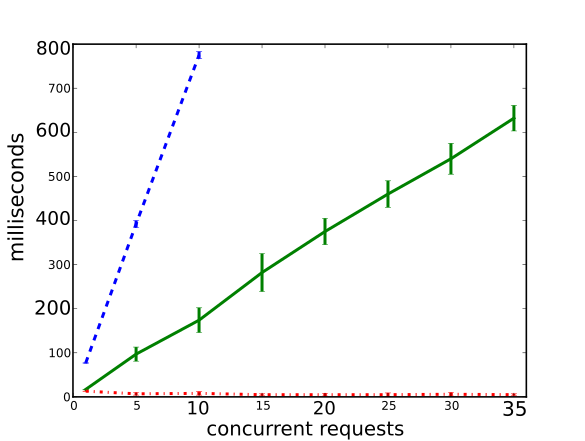
\includegraphics[width=3in]{images/device_comparison.png}
% \label{fig:deviceCompatison}
% \caption{Time measurement comparison among XBee sensors, FoxG20 and a regular computer}
% \end{figure}




\InsertFig{device_comparison}{fig:deviceComparison}{
  Response times measured in different embedded devices
}{
  The dash-dotted line represents the regular computer, the solid line the FoxG20 and the dashed line the XBee.
}{0.7}{}


\begin{table}[htbp]
    \caption{Mean of the measurements taken in different devices with the standard deviation ($\sigma$) in parenthesis.}
    \centering
    \begin{tabular}{|c|c|c|c|}
      \hline
      Concurrent & XBee & FoxG20 & Regular \\
      requests   &  & &  computer \\
      \hline
      1  &  77 (1)	&  17 (0)  &  13 (0) \\
      5  & 392 (8)	&  97 (16) &   7 (3) \\
      10 & 775 (8)	& 174 (28) &   8 (4) \\
      15 &  -	& 282 (43) &   5 (2) \\
      20 &  -	& 375 (30) &   5 (3) \\
      25 &  -	& 460 (30) &   5 (4) \\
      30 &  -	& 540 (35) &   6 (4) \\
      35 &  -	& 632 (29) &   5 (2) \\
      \hline
    \end{tabular}
    \label{tab:timeMeasures}
\end{table}
\subsection{Application Integration}
\label{sec:soa_integration}

% Definiciones de middleware en el libro de Coulouris:
%
% (pag 17):
% Middleware • The term middleware applies to a software layer that provides a
% programming abstraction as well as masking the heterogeneity of the underlying
% networks, hardware, operating systems and programming languages.
%
% (en otra parte):
% The task of middleware is to provide a higher-level
% programming abstraction for the development of distributed systems and, through
% layering, to abstract over heterogeneity in the underlying infrastructure to promote
% interoperability and portability.


The integration of two applications is driven by how they communicate.
To ease that communication the applications use middlewares.
A middleware is a software layer which provides a higher level of abstraction and masks the underlying heterogeneity.
\citet{coulouris_distributed_2012} define two communication styles on the upper layer of a middleware: % figura 4.1 modificada para incluir elementos
the remote invocation and the indirect communication (see Figure~\ref{fig:middleware_layers}).

\InsertFig{middleware_layers}{fig:middleware_layers}{Middleware layers}{Middleware layers according to \citet{coulouris_distributed_2012} classification.}{1}{}
% According to Coulouris et al. HTTP is An example of a request-reply protocol!


The \emph{remote invocation} involves the most common two-way exchange between senders and receivers in distributed systems.
Within the \emph{remote invocation} style, RESTful style \citep{fielding_architectural_2000} and the well known set of WS-* \citep{alonso_web_2010} standards probably represent the most popular substyles.
In Section~\ref{sec:remote_invocation}, we analyze their application to the \ac{ubicomp} field, particularly focusing on the \ac{iot}.


\medskip


The \emph{indirect communication} style comprehends all the techniques with no direct coupling between the sender and the receiver.
% Otra forma:
% In contrast, the \emph{indirect communication} comprehends decoupled communications between senders and receivers.
The group communication, publish-subscribe systems, message queues or shared memory approaches are examples of indirect communication.
These paradigms are characterized by two key properties \citep{gelernter_generative_1985,coulouris_distributed_2012}
\footnote{
  We use the terminology of the  \aclp{ts}' seminal paper \citep{gelernter_generative_1985}, but please note that:
  % nomenclature, naming or terminology?
  \begin{itemize}
    %\item Gelernter et al. stated that \emph{distributed sharing} was just a consequence of the these properties.
    \item The \emph{space uncoupling} property is referred as \emph{reference autonomy} by some authors \citep{fensel_triple-space_2004}.
	  % El primero fue un tal Angerer en el 2002, pero en un artículo en alemán.
	  % En el 2003 hay un artículo suyo en Internet, pero no sé si mencionarlo.
    \item These authors mention a third property confusingly called \emph{space autonomy} (or \emph{location autonomy}).
	  According to \citet{fensel_triple-space_2004} this autonomy is achieved because:
	  \begin{quote}
	    The processes can run in completely different computational environments as long as both can access the same space.
	  \end{quote}
  \end{itemize}
}
:

\begin{itemize}
 \item \emph{Space uncoupling}, which is achieved when the sender does not need to know the receiver or receivers and vice versa.
 \item \emph{Time uncoupling}, which happens when senders and receivers do not need to exist in the same time\footnote{
	  Although some authors \citep{fensel_triple-space_2004,krummenacher_www_2005} explain this property just in terms of communication asynchrony,
	  % mencionar a otros? o no porque simplemente siguen lo dicho por Fensel?
	  % a Bundler no lo cito, porque era una master thesis "sólo"
	  % en este caso cito a krummenacher porque en esa publicación lo define directamente como el no uso de comunicación sincrona
	  \citet{coulouris_distributed_2012} make a clear distinction between them.
	  In their words, a communication is asynchronous when \emph{a sender sends a message and then continues without blocking},
	  whereas time uncoupling adds an extra dimension: \emph{the sender and the receiver can have independent existences}.
	  }.
 
\end{itemize}

\acl{ts} computing, also called space-based computing, offers an improvement of the shared memory approach.
Whereas the shared memory works at byte-level and accessing to memory addresses,
the \acl{ts} works with semi-structured data which is accessed in an associative manner.
In other words, in \ac{ts} the participants read data specifying patterns of interest.
In Section~\ref{sec:tuplespaces_eoa}, we study the most relevant \acl{ts} solutions proposed for the \acl{ubicomp}.


\subsection{Remote invocation}
\label{sec:remote_invocation}

% TODO definir en algun lado que es REST y que es WS-*???

% De Guinard 2011 rest-vs-ws
% 
% WS-* These services declare their functionality and interfaces in a Web Ser-
% vices Description Language (WSDL) file. Client requests and service response
% objects are encapsulated using the Simple Object Access Protocol (SOAP) and
% transmitted over the network, usually using the HTTP protocol. Further WS-
% * standards define concepts such as addressing, security, discovery or service
% composition. Although WS-* was initially created to achieve interoperability of
% enterprise applications, work has been done to adapt it to the needs of resource-
% constrained devices [10, 13]. Furthermore, lighter forms of WS-* services, such
% as the Devices Profile for Web Services (DPWS)1, were proposed [6].
% 
% REST At the core of a RESTful architecture [3] lie resources that are uniquely
% identified through Uniform Resource Identifiers (URIs). The Web is an imple-
% mentation of RESTful principles – it uses URLs to identify resources and HTTP
% as their service interface. Resources can have several representation formats (e.g.,
% HTML, JSON2 ) negotiated at run time using HTTP content negotiation. In a
% typical REST request, the client discovers the URL of a service it wants to call by
% browsing or crawling its HTML representation. The client then sends an HTTP
% call to this URL with a given verb (GET, POST, PUT, etc.), a number of options
% (e.g., accepted format), and a payload in the negotiated format (e.g., XML or
% JSON). Several recent research projects implement RESTful Web services for
% smart things [2] within what has become to be known as the Web of Things [5].


% De Pautasso 2008
% 
% REpresentational State Transfer (REST) was originally introduc-
% ed as an architectural style for building large-scale distributed hy-
% permedia systems. This architectural style is a rather abstract entity,
% whose principles have been used to explain the excellent scalability
% of the HTTP 1.0 protocol and have also constrained the design of
% its following version, HTTP 1.1. Thus, the term REST very often
% is used in conjunction with HTTP.


As stated before, the RESTful style and the set of WS-* standards are probably the most common remote invocation substyles currently used in the Internet.
Their advantages and disadvantages were extensively discussed by \citet{pautasso_restful_2008}.

WS-* standards syntactically describe the services' functionality and interfaces using \ac{wsdl}.
The communication between providers and consumers is usually transmitted over the \ac{http} in messages encapsulated using \ac{soap}.
WS-* web services, also called ``Big Web services'', offer more features such as transactions, reliability or message-level security.
However, they also require further architectural decisions on different layers of the WS-* stack.
These decisions make the people perceive it as more complex than the RESTful style \citep{guinard_search_2011}.


Probably thanks to that perception, \ac{rest} has gained momentum during the last decade. %  simpler alternative for services
% la explicación de los principios los he sacado sobre todo de pautasso_restful_2008, pero he intentado no plagiar las frases.
The \acl{rest} is defined by four principles \citep{fielding_architectural_2000}:
\begin{enumerate}
  \item The resources are identified with \acp{uri}.
  \item They are manipulated through a uniform interface.
	  This interface offers creation, reading, updating and deletion operations.
  \item The resources are decoupled from their representation so the content can be accessed in different formats.
  \item The interactions are stateful and hypertext-driven.
	This means that the state transitions are guided by the actions identified in the hypermedia by the server.
	% De Wikipedia: This means that clients make state transitions only through actions that are dynamically identified within hypermedia by the server.
\end{enumerate}

These principles are implemented by the Web,
so \ac{rest}  is often used in conjunction with well-known web standards such as \ac{http}, \ac{uri} or \ac{mime}.
This standards already have many libraries and tools available, which eases the adoption of this style by developers.
Besides, REST naturally integrates with the \ac{www} because it uses the Web as an application architecture instead of as a transport layer as WS-* services do.
% ojo a la frase: "se integra con la web porque usa la web como app architecture"

\bigskip


The use of both substyles in resource-constrained devices is represented by
\ac{dpws} \citep{moritz_devices_2010}, based on WS-*,
and the \ac{wot} \citep{guinard_internet_2011}. % o mejor poner su tesis?


\InsertFig{venn-sec1_1}{fig:venn_ubicomp}{
  Non-semantic integration approaches for \ac{ubicomp} apart from \aclp{ts}.
}{
  Scope of this subsection.
}{0.6}{}


\ac{dpws} defines a subset of WS-* to make it suitable for resource-constrained devices.
%\ac{dpws} is claimed to be used in industrial environments.
Its most remarkable features are: decentralized multicast-based discovery, secure message transmission, subscription and event notifications.
\citet{moritz_devices_2010} compared \ac{dpws} with the \ac{rest} approach coming to the conclusion that \ac{dpws} can be restricted to be fully compatible with the RESTful style.
Even in that case, \ac{dpws} will still cover some missing features of the RESTful approach such as eventing and discovery \citep{moritz_devices_2010}.
% no menciono que sean más pesados para cacharros porque no he encontrado un sitio en el que defiendan que \ac{dpws} lo es (si que hay alguno que comparan REST y SOA, pero no DPWS)


The \acl{wot} initiative encourages the use of \acs{rest}-based solutions embedding web servers in daily objects \citep{guinard_internet_2011}.
In this way, the objects can integrate with the \ac{www} as first-class citizens. % decir ``f-c cit of the Web" es reiterativo ya que WWW==web
This integration brings the following benefits:
\begin{itemize}
  \item The smart-things can be linked to enable its discovery by browsing. This involves using the tool most users are familiar with: the browser.
  \item They can be bookmarked or shared through social networks \citep{guinard_sharing_2010}.
  % explicar qué es un mashup?
  \item They can be integrated with other web applications through mash-ups \citep{guinard_towards_2009,ostermaier_webplug:_2010,pintus_anatomy_2011}.
  % TODO citar al canadiense tb? pintus, stirbu y a todo el mundo
  \item Mechanisms such as searching, caching, load-balancing and indexing can be used over the objects to achieve the scalability of the web. % cita al indio
\end{itemize}


% lo he comentado antes, no sé si no me estoy repitiendo más que el ajo...
But besides the functional differences, one of the major advantages of REST compared with the WS-* is that is perceived as simpler.
\citet{guinard_search_2011} proved that developers consider it easier to learn and find it more suitable for programming smart things.
This makes \ac{wot} solutions more popular for resource constrained devices than the WS-* based ones.

% Mencionar un par de trabajos sobre móviles con servidores web embebidos, para que se vea que no es sólo \ac{wot}


% mencionar CoAP y demás protocolos?
% A prove of this success/popularity is the raise of new protocols...
% \ac{wot} has been leveraged to run in devices as constrained as the ones from the Wireless Sensor Networks.
% The special needs of this kind of sensors has brought the need of new protocols such as CoAP which try to adapt HTTP to UDP environments.

% necesita comparativa esta parte?
\subsection{\acl{ts}}
\label{sec:tuplespaces_eoa}

% Ojo cuidado porque según esto mi middleware va a dejar de ser time uncoupled! (mirar Figure 6.1 para mayor concrección)
% En esa misma sección aclara que algunas implementaciones no son time-uncoupled.
% por otro lado, asíncronismo != time uncoupling

\acf{ts} has its roots in the Linda parallel programming language \citep{gelernter_generative_1985}.
In this communication model different processes read and write pieces of information so-called tuples in a common space.
Tuples are composed by one or more typed data fields (e.g. $<"aitor",1984>$ or $<3,7,21.0>$).
The tuples are accessed associatively using a template.
A template provides either a value or type for different fields (e.g. $<String,1984>$ or $<Integer, Integer, Float>$).
The operations over the space are defined by different primitives.
Although the primitives may change from implementation to implementation, the most common ones allow to:

\begin{itemize}
  \item \emph{Access the tuples non-destructively}, using a primitive which is usually called \emph{read} or \emph{rd}.
	This primitive returns a tuple from the space which matches the given template without changing the space.
  \item \emph{Access the tuples destructively}, using a primitive which is usually called \emph{take} or \emph{in}.
	This primitive extracts a tuple which matches the given template from the space.
  \item \emph{Write a new tuple into the space}. This primitive is usually called \emph{write} or \emph{out}.
\end{itemize}


\InsertFig{venn-sec1_2}{fig:venn_tuplespaces_ubicomp}{
  \aclp{ts} solutions for Ubicomp.
}{
  Scope of this subsection.
}{0.6}{}

\bigskip

% Ignorar esta sección? Es realmente necesaria cuando ya he puesto la comparativa de TSC?
So far, \acl{ts} has been adapted to \acl{ubicomp} by different authors.

% TODO leer artículos que me faltan y corregir
The \emph{event heap} \citep{johanson_extending_2004} is a system used for a specific \ac{ubicomp} sub-domain: interactive workspaces.
In this scenario there are rooms with different devices deployed and where mobile devices can enter.
Each room has its own space where the devices exchanging tuples to cooperate.
%For example, a video can be presented in a display and through a remote controller, the user can place the tuple for pausing it.
%The display consumes these kind of tuples, so it pauses the video whenever somebody places that tuple on the space.
% This system is simple to implement but is limited since it centralizes the space in a single machine per room.
This work merely identifies the requirements of these environments and the properties which solve them.
Then, it discusses how these properties can be satisfied using \ac{ts} or some extensions.
Finally they compare its implementation both with other \acp{ts} implementations or other coordination infrastructures. % e.g. RMI, MOM, Pub/sub

Although the analysis presented by \citeauthor{johanson_extending_2004} identifies the key requirements for \ac{ts} in \ac{ubicomp},
the solution they propose is purely centralized.
We opted for a distributed solution at the expense of limiting some of the features.
% indicar cuales son o pasar?
% usar sus características a la hora de valorar nuestra solución TSC en futuras secciones?


\emph{L$^2$imbo} \citep{davies_l2imbo:_1998,friday_experiences_1999} replicates the tuples to avoid a single point of failure.
Each node joined to a space uses an IP multicast address to exchange messages with other nodes in that space.
Writing into a space involves sending a multicast message to inform to the rest of the nodes of the tuple written.
Reading operation usually requires local reading.
Destructive reading of the tuple is more complex as it requires a global withdrawal.
In \emph{L$^2$imbo} only the owner of a tuple can remove it from the space.
The ownership of a tuple initially belongs to its creator, but can be transferred. % TODO ver qué añadió Friday


 % meter mas citas de LIME que estas 2?
\emph{LIME} (Linda in a Mobile Environment) \citep{picco_lime:_1999} is a TS solution for mobile systems.
In LIME each mobile device has its own space where it generally writes its tuples.
This space is shared with other devices creating federated spaces, i.e. the aggregation of different shared spaces.
In this way, each mobile can access to tuples in other mobiles whenever they become available.
They also proposed a new writing primitive to insert tuples in remote spaces.
% ejemplo de service discovery?

This is difficult to implement and \citet{coulouris_distributed_2012} complain about the unrealistic assumptions they make to simplify the problem. % cita al libro
These assumptions are the uniform multicast connectivity between devices whose tuple spaces are aggregated and the serialized and ordered connections and disconnections.
In any case, LIME was adapted to several platforms to run both in embedded and mobile devices \citep{murphy_transiently_2006}.


In the \emph{TOTA} (Tuples On The Air) Project \citep{mamei_programming_2009} tuples are disseminated to different devices.
To that end, each tuple has 3 fields:
1) the content of the tuple,
2) a rule which defines how it should be propagated,
3) a rule to define its maintenance.
For instance, they consider a museum where a visitor writes a query tuple describing a piece of art he wants to see.
The propagation rule defines that it should be propagated to all nodes in the vicinity, increasing the distance by one each time.
The tuple is configured to be deleted after a time-to-live period using its maintenance rule.
When the it reaches the room where the piece of art is located, the piece of art will write a response tuple.
This response tuple jumps from a device to another until it reaches the device which queried for it.


% TODO Analizar otras como TOTAM o CRIME
\subsection{Looking for Application-level Interoperability}
\label{sec:soa_sw}
% centrarse en el ejemplo de interoperabilidad d nivel de aplicaciones
% TODO reducir este rollo infame de intro

A common problem in most of the \ac{ubicomp} solutions is the use of application domain dependent data formats.
% learn about the data-schema, learn about the syntax and the meaning??? mirar cómo lo explican en otros lados
These formats require developers of new applications to learn about the syntax and the meaning of that data in order to be able to reuse that information.

Section~\ref{sec:semantic_web} presents how the \acl{sw} tackles these problems.
Sections~\ref{sec:sw_intermediaries}~and~\ref{sec:sw_providers} analyze some remarkable works within the \ac{ubicomp} field which use the \ac{sw}.


\subsection{The \acl{sw}}
\label{sec:semantic_web}

A problem of the initial view of the Web was that it was human-centered.
Regardless of whether the contents were machine processable, a human needed to interpret them to give them a meaning.
% mirar a ver cuando se empezó a usar SW de verdad, porque en el artículo de 2001 dan a enterder que se llevaba un tiempo usando
In the early 2000s, \citet{berners-lee_semantic_2001} proposed the use of what they called the \acf{sw} to solve that problem.
The SW was conceived as an extension of the ordinary web which would bring structure to its content.
As the ordinary web, the SW benefits from the universality the hypertext provides by linking \emph{anything with anything}.
Besides, like the Internet, the SW is intended to be as decentralized as possible.

The \acl{sw} and its key features are defined by the \emph{World Wide Web Consortium} \citep{semanticWeb-FAQ} as:
\begin{quote}
The vision of the \acl{sw} is to extend principles of the Web from documents to data.
Data should be accessed using the general Web architecture using, e.g., URI-s;
data should be \emph{related to one another} just as documents (or portions of documents) are already.
This also means creation of a common framework that allows data to be \emph{shared and reused} across application, enterprise, and community boundaries,
to be \emph{processed automatically} by tools as well as manually, including revealing possible \emph{new relationships} among pieces of data.
\end{quote}

Meaning is expressed in the \acl{sw} as sets of triples.
Each triple is composed by a subject, a predicate and an object like in a normal sentence (see Figure~\ref{fig:triples_example}).
Therefore, in  \citeauthor{berners-lee_semantic_2001} words, \emph{a document can assert that things (people, web pages or whatever) have properties (such as "is a sister of," "is the author of") with certain values (another person, another Web page)}.
A key difference with a normal sentence is that each concept is unambiguously defined by an URI.
These URIs form links between different triples as shown by the example of the Figure~\ref{fig:triples_example}.
% This set of triples can be expressed in multiple formats such as RDF, Turtle, Notation3 or NTriples. % TODO citas


\InsertFig{triples_example}{fig:triples_example}{
  Sample triples using different ontologies.
}{
  All the triples are represented graphically and some of them also textually.
  They describe academic and personal details about the author of this thesis.
  The knowledge is expressed using four different ontologies: FOAF, DC, SWRC and CiTE. % citar?
  Note that we use aliases, known as prefixes in most Semantic formats, to shorten some URIs and enhance the clarity of the Figure.
}{1}{}


A problem with the information described so far is that two different databases may use different URIs to express the same concept.
To overcome this the \ac{sw} offers collections of information called ontologies.
An ontology is a document which expresses the relations between terms commonly using a taxonomy and a set of rules to infer content.
The taxonomy defines the classes of a given domain and how they relate with each other.

Of course, different content providers could provide similar data described according to different ontologies.
Fortunately, ontologies can be easily mapped by providing equivalence relations within them.
In the same way, an ontology can be extended to adapt it to different application domains.
In any case, the reuse of the same models is beneficial and is therefore promoted through standardization.

% Remarkably, the use of the \ac{sw} has been promoted in the last years with the Linked Open Data (LOD) initiative.
% The LOD are datasets which follow a series of principles on how to open and publish data.
% The ultimate goal of the LOD is to publish linked terms using full semantics.
\subsection{Conclusions} % or Discussion???


In Section~\ref{sec:remote_invocation} we have analyzed the current trends towards the remote invocation style.
Within them, we can see how \ac{wot} has gained much more attention both for its perceived simplicity and for its seamless integration with the web.
% o decir REST based solutions para no centrar mucho en IoT
Besides, the availability of tools and libraries for many mobile and embedded platforms ease its adoption.


However, as any remote invocation style it introduces coupling between senders and receivers.
% de johanson_extending_2004 he sacado esas características, no la particularización a WoT
These complicates the application changes both in the short-term and in the long-term \citep{johanson_extending_2004}.
In the short-term because nodes constantly join and leave the environment due to mobility or to failures.
In the long-term because the space is used to solve new problems and the obsolete devices are replaced with new technology.
Furthermore, the human interaction is eased by minimizing the configurations.
% quizá lo de johanson_extending_2004 se podría retomar en el capítulo cha:tsc
In Chapter~\ref{cha:tsc}, we deeply compare both \ac{rest} and \ac{ts} to see how they can benefit each other.


\bigskip


% comparación de todas ellas
% de entre los que ofrecen distribución: este no mola por esto, esto otro mola por esto otro, etc.

In Section~\ref{sec:remote_invocation} we have studied the \ac{ts} solutions for \acl{ubicomp}.
Within these solutions, \emph{The event heap} is not considered because of its centralized nature.
The rest present different ways to disseminate the tuples. %  L2imbo, LIME and TOTA

The replication which L$^2$imbo proposes may not be feasible for devices with constrained memory or storage capacity.
Particularly, in spaces populated by many devices like the Internet of Things a large amount of tuples can be generated.
% need to configure the network

TOTA is useful for spatially connected \emph{ad hoc} environments, but it does not seem to suit well on networks where all the nodes can reach each other.
In this case, all the tuples could be replicated on the rest of the nodes showing the same limitations as L$^2$imbo.
% TODO COMPROBAR LEYENDO CON ATENCION LO DE TOTA!!!
Furthermore, \emph{ad hoc} environments are not the focus of our solution since we assume the connectivity between all the devices in a space.

% TODO no darle tan duro que si no a ver como luego me comparo con ellos :-)
Finally, despite of their unrealistic assumptions LIME proposes a model where each tuple is responsible of its own part of the space.
They share spaces whenever they become available.


\begin{table}%[position specifier]
  \centering
  \begin{tabular}{ c | c c c c }%p{5cm}}
      ~ & The event heap & L2imbo & LIME & TOTA \\
      \hline
      Distributed & No & Yes & Yes & Yes \\
      Objective & - & Availability & Federation & Ad-hoc \\
      % Scalability?
      % Coger propiedades del libro de sistemas distribuidos?
  \end{tabular}
  \caption{Comparison of the most prominent \acl{ts} alternatives for \acl{ubicomp}.} % no columpiarme, o poner todas o ninguna?
  \label{tab:ubicomp_ts_comparison}
\end{table}


\medskip

In our model, we argue that in an \ac{ubicomp} environment each node should manage their own semantic information.
By delegating responsibility 
we naturally represent mobility scenarios where users carry their own profiles in their mobiles to new spaces 
and 
we acknowledge the fact that embedded devices directly control their own actuators and sensors.
Therefore, we propose to directly access to the source of the data avoiding the use of intermediaries whenever it is possible.
In this aspect, our solution has more in common with LIME.
Two major differences with LIME are the use of semantics and the natural integration with the web. % i.e. use of REST/HTTP